%%%%%%%%%%%%%%%%%%%%%%%%%%%%%%%%%%%%%%%%%%%%%%%%%%%%%%%%%%%%%%%%%%%%%%%%
%%%  THIS TEX FILE IS TO GENERATE PDF FILE FOR 
%%% 
%%%  COPYRIGHT (C) JIMMY LIN, 2013, UT AUSTIN
%%%%%%%%%%%%%%%%%%%%%%%%%%%%%%%%%%%%%%%%%%%%%%%%%%%%%%%%%%%%%%%%%%%%%%%%
\documentclass[11pt,a4paper]{article}
%%%%%%%%%%%%%%%%%%%%%%%%%%%%%%%%%%%%%%%%%%%%%%%%%%%%%%%%%%%%%%%%%%%%%%%%
%%%  PACKAGES USED IN THIS TEX SOURCE FILE
%%%%%%%%%%%%%%%%%%%%%%%%%%%%%%%%%%%%%%%%%%%%%%%%%%%%%%%%%%%%%%%%%%%%%%%%
\usepackage{geometry,amsthm,amsmath,graphicx,amssymb,fancyheadings}
\usepackage[]{mcode}
\usepackage[colorlinks,
            linkcolor=blue,
            anchorcolor=red,
            citecolor=green
            ]{hyperref}
% for my mac
\IfFileExists{/Users/JimmyLin/.latex/UTA_CS/JS.sty}{ 
    \usepackage{/Users/JimmyLin/.latex/UTA_CS/JS}
    \usepackage{/Users/JimmyLin/.latex/UTA_CS/JSASGN}
}{} 
% for UT's linux machine
\IfFileExists{/u/jimmylin/workspace/Configs/latex/UTA_CS/JS.sty}{
    \usepackage{/u/jimmylin/.latex/UTA_CS/JS} 
    \usepackage{/u/jimmylin/.latex/UTA_CS/JSASGN}
}{} 
%%%%%%%%%%%%%%%%%%%%%%%%%%%%%%%%%%%%%%%%%%%%%%%%%%%%%%%%%%%%%%%%%%%%%%%%
%%% MACROS CONTAINING THE FILE INFORMATION
%%%%%%%%%%%%%%%%%%%%%%%%%%%%%%%%%%%%%%%%%%%%%%%%%%%%%%%%%%%%%%%%%%%%%%%%
\renewcommand{\COURSE}{EE381V Large Scale Optimization}
\renewcommand{\LECTURER}{Sujay Sanghavi}
\renewcommand{\SECTION}{17350}
\renewcommand{\TASK}{Problem Set 1}
\renewcommand{\RELEASEDATE}{September 12, 2014}
\renewcommand{\DUEDATE}{September 18, 2014}
\renewcommand{\TIMECONSUME}{10 hours}
%%%%%%%%%%%%%%%%%%%%%%%%%%%%%%%%%%%%%%%%%%%%%%%%%%%%%%%%%%%%%%%%%%%%%%%%
%%% DOCUMENTATION STARTS FROM HERE 
%%%%%%%%%%%%%%%%%%%%%%%%%%%%%%%%%%%%%%%%%%%%%%%%%%%%%%%%%%%%%%%%%%%%%%%%
\begin{document}
%%%%%%%%%%%%%%%%%%%%%%%%%%%%%%%%%%%%%%%%%%%%%%%%%%%%%%%%%%%%%%%%%%%%%%%%
%% TITLE PAGE
%%%%%%%%%%%%%%%%%%%%%%%%%%%%%%%%%%%%%%%%%%%%%%%%%%%%%%%%%%%%%%%%%%%%%%%%
\begin{titlepage}
    \maketitle
\end{titlepage}
%%%%%%%%%%%%%%%%%%%%%%%%%%%%%%%%%%%%%%%%%%%%%%%%%%%%%%%%%%%%%%%%%%%%%%%%
%% CONTENT PAGE: TABLEOFCONTENTS, LISTOFTABLES, LIST OF FIGURES
%%%%%%%%%%%%%%%%%%%%%%%%%%%%%%%%%%%%%%%%%%%%%%%%%%%%%%%%%%%%%%%%%%%%%%%%
\renewcommand{\contentsname}{Table of Contents}
\begin{center} 
    \tableofcontents 
    %\listoftables 
    \listoffigures
\end{center}
\newpage
%%%%%%%%%%%%%%%%%%%%%%%%%%%%%%%%%%%%%%%%%%%%%%%%%%%%%%%%%%%%%%%%%%%%%%%%
%%% GENERAL DOCUMENTATION BEGINS 
%%%%%%%%%%%%%%%%%%%%%%%%%%%%%%%%%%%%%%%%%%%%%%%%%%%%%%%%%%%%%%%%%%%%%%%%

\section{Matlab and Computational Assignment}
\subsection{Gradient Descent on three matrices}
Command to get executed: 
\begin{verbatim}
   >> gd_run_script()
\end{verbatim}
\subsubsection{$X1$, $b1$}
\begin{itemize}
    \item Range of $\gamma$ that leads to convergence: $(0,2)$
    \item Range of $\gamma$ that leads to divergence: $(2,+\infty)$
    \item Explanation: if $\gamma = 2$, the program indicates that 
        $$ \forall k,\ f(x^{k+1}) = f(x^{k})$$ 
        Since the above equation is constantly true (independent of the
        minima), we can conclude that gradient descent with $\gamma = 2$ goes 
        to the opposite side of that quadratic curve. Intuitively, the program 
        will diverge if we set larger ($\gamma>2$) and converge if we set smaller
        ($\gamma<2$).   
    \item Two illustrative examples: $\gamma = 0.5$ and $\gamma = 3.0$
        \begin{figure}[h]
            \centering
            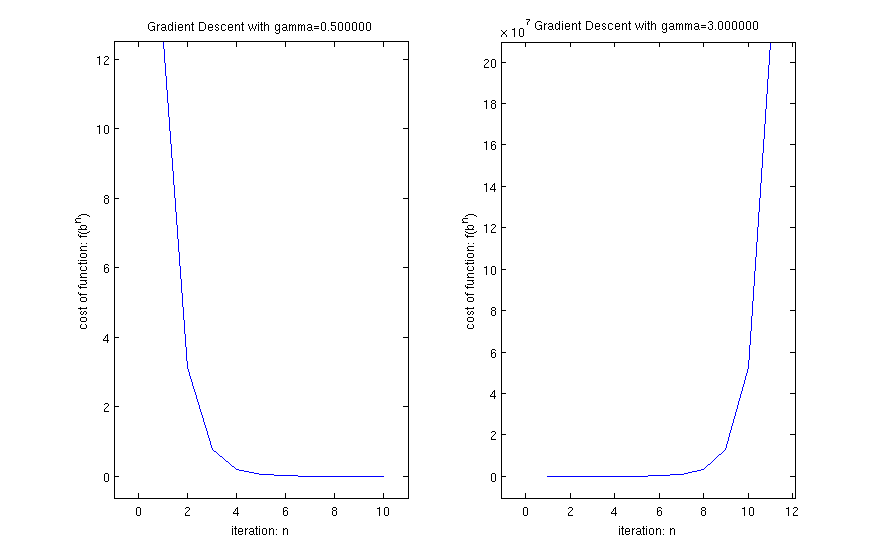
\includegraphics[width=6in,height=3in]{../ps1_matlab/1.png}
            \caption{Illustration for gradient descent on $X1$, staring with
                $b1$ by $\gamma = 0.5$ and $3.0$}
        \end{figure}
\end{itemize}

\newpage
\subsubsection{$X2$, $b2$}
\begin{itemize}
    \item Range of $\gamma$ that leads to convergence: $(0,2)$
    \item Range of $\gamma$ that leads to divergence: $(2,+\infty)$
    \item Explanation: if $\gamma = 2$, the program indicates that 
        $$ \forall k,\ f(x^{k+1}) = f(x^{k})$$ 
        Since the above equation is constantly true (independent of the
        minima), we can conclude that gradient descent with $\gamma = 2$ goes 
        to the opposite side of that quadratic curve. Intuitively, the program 
        will diverge if we set larger ($\gamma>2$) and converge if we set smaller
        ($\gamma<2$).
    \item Two illustrative
        examples: $\gamma = 1.5$ and $\gamma = 3.0$
        \begin{figure}[h]
            \centering
            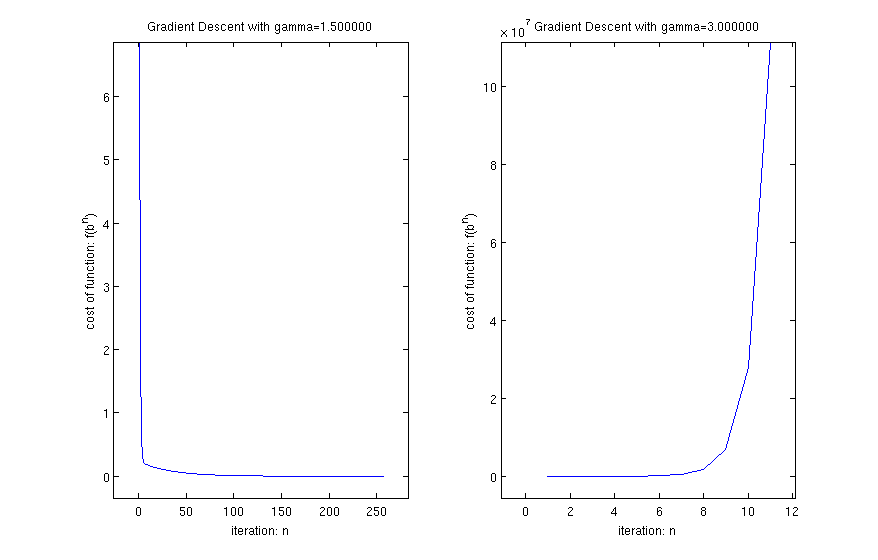
\includegraphics[width=6in,height=3in]{../ps1_matlab/2.png}
            \caption{Illustration for gradient descent on $X2$, starting with
                $b2$ by $\gamma = 1.5$ and $3.0$}
        \end{figure}
\end{itemize}

\newpage
\subsubsection{$X3$, $b3$}
\begin{itemize}
    \item Range of $\gamma$ that leads to convergence: $(0,0.02)$
    \item Range of $\gamma$ that leads to divergence: $(0.02,+\infty)$
    \item Explanation: if $\gamma = 0.02$, the program indicates that 
        $$ \forall k,\ f(x^{k+1}) = f(x^{k})$$ 
        Since the above equation is constantly true (independent of the
        minima), we can conclude that gradient descent with $\gamma = 0.02$ goes 
        to the opposite side of that quadratic curve. Intuitively, the program 
        will diverge if we set larger ($\gamma>0.02$) and converge if we set smaller
        ($\gamma<0.02$).
    \item Two illustrative examples: $\gamma = 0.005$ and $\gamma = 0.05$
        \begin{figure}[h]
            \centering
            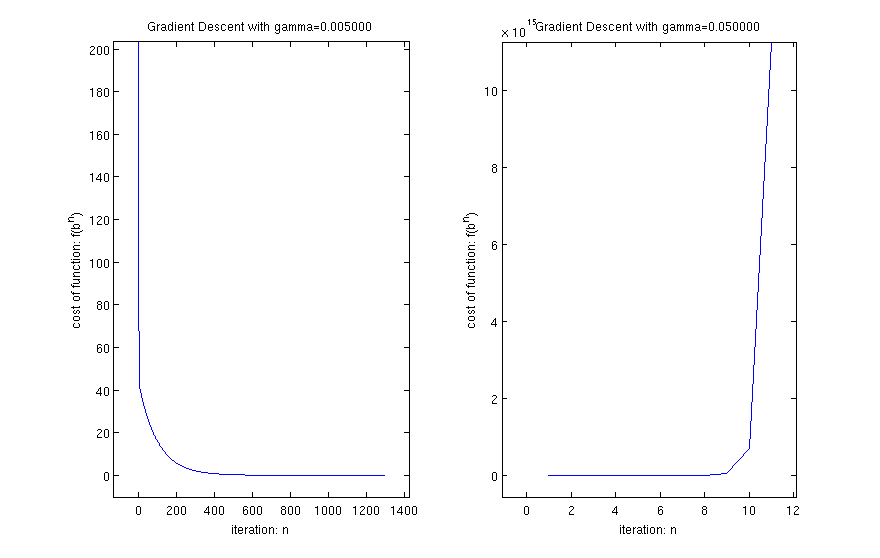
\includegraphics[width=6in,height=3in]{../ps1_matlab/3.png}
            \caption{Illustration for gradient descent on $X3$ staring with
                $b3$ by $\gamma = 0.005$ and $0.05$}
        \end{figure}
\end{itemize}

\newpage
\subsection{$\gamma = 1$ for the second matrix}
Command to get executed: 
\begin{verbatim}
   >> [b2_opt, iters, all_costs] = Gradient_Descent(X2, b2, 1);
\end{verbatim}
{\bf Plotting}: figure for $\gamma = 1$
\begin{figure}[h]
            \centering
            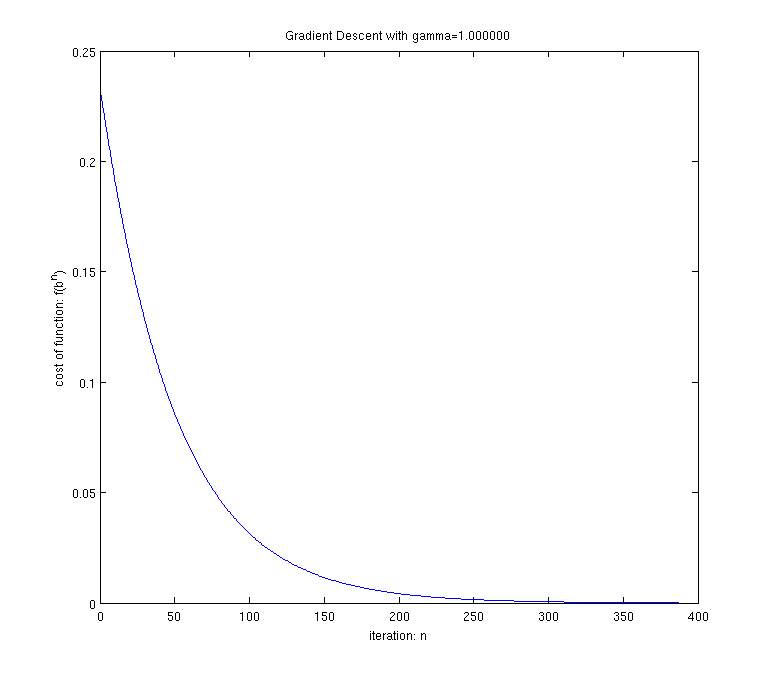
\includegraphics[width=4in,height=3in]{../ps1_matlab/2_gamma1.png}
            \caption{Plotting figure for gradient descent with $\gamma = 1$ on
            the second matrix}
\end{figure}

\noindent
{\bf Explanation}: 
Through the smooth plotted curve, we guess that the gradient
descent method got linear convergence when $\gamma=1$ on $X_2$. Hence, we trace
convergence rate conv\_rate $ = f(x^{k}) / f(x^{k-1})$ as follows:
\begin{verbatim}
Iter: 2, Cost: 2.254428e-01, Conv_Rate: 1.020304
Iter: 3, Cost: 2.209565e-01, Conv_Rate: 1.020304
Iter: 4, Cost: 2.165594e-01, Conv_Rate: 1.020304
Iter: 5, Cost: 2.122499e-01, Conv_Rate: 1.020304
Iter: 6, Cost: 2.080261e-01, Conv_Rate: 1.020304
Iter: 7, Cost: 2.038864e-01, Conv_Rate: 1.020304
...
...
Iter: 384, Cost: 1.043098e-04, Conv_Rate: 1.020304
Iter: 385, Cost: 1.022340e-04, Conv_Rate: 1.020304
Iter: 386, Cost: 1.001996e-04, Conv_Rate: 1.020304
Iter: 387, Cost: 9.820558e-05, Conv_Rate: 1.020304
\end{verbatim}
In terms of above dumps and the fact that $f(x^{*}) = 0$, we can conclude that when $\gamma = 1$        
$$
f(x^{k+1}) - f(x^{*}) = 1.020304 \cdot \big( f(x^{k}) - f(x^{*}) \big)
$$

\newpage
\section{Written Problems}
\subsection{Orthogonal Subspaces}
\subsection{Boyd and Vandenberghe, Ex. 2.10}
\subsection{Boyd and Vandenberghe, Ex. 2.21}
\subsection{Form a Half-Space}
\subsection{Exists $C$ s.t. $CA = B$}

\newpage
\appendix
\section{Codes Printout}

\subsection{Gradient Descent Routine}
\lstinputlisting{../ps1_matlab/Gradient_Descent.m}
\newpage

\subsection{Running Script}
\lstinputlisting{../ps1_matlab/gd_run_script.m}

%%%%%%%%%%%%%%%%%%%%%%%%%%%%%%%%%%%%%%%%%%%%%%%%%%%%%%%%%%%%%%%%%%%%%%%%
%%% General Documentation ends
%%%%%%%%%%%%%%%%%%%%%%%%%%%%%%%%%%%%%%%%%%%%%%%%%%%%%%%%%%%%%%%%%%%%%%%%
\end{document}
